This chapter contains a detailed description of each of the system functionalities; including the algorithms and implementations.
\label{chapter_methdology}


%-----------------------------------------------------%

\section{Autonomous Functionalities}
\label{method_auto_func}
This section highlights the implementation of our AV's autonomous functionalities. Each subsection presents the algorithmic details of the corresponding section previously discussed in \ref{specs_auto_func}.

\subsection{Mapping and Localization}
\label{method_loc_map}
As highlighted in \ref{specs_loc_map}, we adopt gmapping and AMCL as our algorithms for implementing the the mapping and localization functionalities of our AVs. This sub-section describes our implementation in more detail.
\begin{enumerate}
\item \textbf{Mapping} 
\\ 
Our map was created manually by moving the vehicle throughout the world using the keyboard, it was find that spawning the vehicle near the origin of the world will result in a better map during the mapping process.
Usually creating maps with normal gmapping package can generate a map that has some defauts and needs to be improved to achieve better results further. One way to edit the map is to manually edit it using GIMP software \cite{gimp}; a photo editor software that supports .pgm extensions.\\
\item \textbf{Localization} 
\\
We use AMCL package in localization, it takes the generated map as an input and tries to localize the the vehicle in it. One of the most important parameters is the number of particles where we chose to use to default configuration for this parameter; min\_particles = 500 and max\_particles = 2000. Also, Default configuration were used in all other parameters.\\
\end{enumerate}

%-----------------------------------------------------%
\subsection{Longitudinal Control}
\label{method_long_ctrl}
In this subsection, we explain our implementation of the Krauss model, previously discussed in \ref{specs_long_ctrl}, whose intended output is the velocity for the vehicle to undertake at each time step. This output velocity is then mapped to the required throttle output as in\cite{f110-fall2018-skeletons}, and then passed through a simple proportional (P) controller to issue the appropriate final control action. \\ \\
The inputs and needed parameters of our Krauss model are as follows:

\begin{itemize}
    \item \textbf{Inputs:}
        \begin{enumerate}
            \item \textbf{Vehicle Position:} This is obtained from the vehicle’s LiDAR sensor.
            \item \textbf{Vehicle Velocity:} This is obtained from the vehicle’s electronic speed controller (ESC).
            \item \textbf{List of Other Vehicles’ IDs:} This is the list of  IDs received, through V2V communication (see \ref{method_v2v_comm}), from all other vehicles within the vehicle’s communication range. This is needed in order for our vehicle to be able to determine which vehicle, if any, is its leading vehicle and to save its data for use in calculations.
        \end{enumerate}
    \item \textbf{Parameters:}
        \begin{enumerate}
            \item \textbf{Vehicle Maximum Velocity}
            \item \textbf{Vehicle Maximum \& Minimum Acceleration}
            \item \textbf{Vehicle Length:} In case a lead vehicle is found, this is needed in order to properly calculate the current gap between the follow and the lead vehicles. This parameter is assumed to be a standard set for all vehicles; i.e. all vehicles have the same length.
            \item \textbf{Safety Inflation Factor:} This parameter is given as a percentage of the vehicles’ length. It defines a value with which to inflate the actual length of the vehicles to be used in calculations; for the sake of increased safety. 
            \item \textbf{Lane Numbering Convention:} This is the convention of the lane numbering in the current map. It is needed in order for the vehicle to map its position coordinates to a lane number.
            \item \textbf{Average Reaction Time:} In case of the presence of a lead vehicle, this is an estimated value for the time our vehicle takes to respond to a sudden change in the lead vehicle's behavior. It reflects on the gap our vehicle seeks to keep between the lead vehicle and itself.
            \item \textbf{Delta Time:} This parameter specifies the time interval between iterations of the Krauss model in which it calculates and outputs the required velocity.
        \end{enumerate}
\end{itemize} 
Using these inputs and specified parameters, the Krauss model calculates the desired velocity every delta time using the following steps:

\begin{enumerate}
    \item With the lane numbering convention and the vehicle’s coordinates in the map being known to the vehicle, the vehicle’s lane number is calculated.
    \item The model checks which of the other vehicles, if any, is a lead vehicle with respect to our vehicle. This is done by traversing through the communicated list of ID messages belonging to vehicles in the communication range, and checking which of them is ahead of our vehicle in the same lane. Of vehicles satisfying this condition, the closest one to our vehicle is considered our lead vehicle at the time, and its relevant data is stored to be used in calculations.
    \item If a lead vehicle is found, the current gap between the two vehicles is calculated \cite{Krau1998MicroscopicMO}. This is the actual physical distance from the front edge of our vehicle to the rear edge of the lead vehicle after adding the specified inflation to their lengths. Since all the provided vehicle coordinates are of the vehicles' centers, the gap \((g)\) is calculated using equation \ref{krauss_gap}, where \(x_l\) and \(x_f\) are the x-coordinates of the lead and follow vehicles respectively, \(f_{si}\) is the safety inflation factor and \(l\) is the length of the vehicle.
    \begin{equation}
        g = x_l - x_f - (1 + f_{si})*l
        \label{krauss_gap}
    \end{equation}
    \label{gap_pt}
    
    \item Next, the maximum safe velocity with respect to the lead vehicle is to be calculated. This safe velocity is the one which guarantees that, under all circumstances and despite any extreme behavior that might be adopted by the lead vehicle, our follow vehicle can be brought to a complete stop without colliding with the lead vehicle \cite{Krau1998MicroscopicMO}. In other words, this means that the total of the distance to be travelled by our follow vehicle while still reacting to the lead vehicle’s actions and the distance to be taken by our vehicle to completely stop should be less than or, at the least, equal to the total of the current gap between vehicles and the distance to be taken by the lead vehicle to halt. This is demonstrated in equation \ref{krauss_inequal} \cite{Krau1998MicroscopicMO}, where \(v_l\) and \(v_f\) are the velocities of the lead and follow vehicles respectively, \(d(v)\) is the needed braking distance to stop a vehicle travelling with velocity \(v\), \(g\) is the gap calculated in \ref{gap_pt} and \(\tau\) is our follow vehicle’s average reaction time.
    
    \begin{equation}
        d(v_f) + v_f\tau \leq d(v_l) + g
        \label{krauss_inequal}
    \end{equation}
    
    Assuming both vehicles use their maximum deceleration, \(b_{max}\), in order to halt, equation \ref{krauss_inequal} can be re-written as equation \ref{krauss_quadr}, and solved for the maximum \(v_f\) which resembles the maximum possible safe velocity with respect to the lead vehicle.
    
    \begin{equation}
        \frac{v_f^2}{2b_{f_{max}}} + v_f\tau \leq \frac{v_l^2}{2b_{l_{max}}} + g
        \label{krauss_quadr}
    \end{equation}
    \label{safe_vel_pt}
    
    \item Another consideration that might limit the value of the velocity outputted by the model is that neither of our vehicle’s velocity or acceleration should be allowed to exceed its maximum value. Consequently, the final output velocity in case of the presence of a lead vehicle is as calculated in equation \ref{krauss_final_lead} \cite{Krau1998MicroscopicMO}, where \(v_k\) is the velocity outputted by the Krauss model, \(v\) is our vehicle's current velocity, \(v_{max}\) and \(a_{max}\) are its maximum velocity and acceleration respectively, \(\Delta t\) is the specified delta time parameter, and \(v_{safe}\) is the maximum safe velocity calculated in \ref{safe_vel_pt}.

    \begin{equation}
        v_k(t) = min(v_{max}, (v(t) + a_{max}*\Delta t), v_{safe}(t))
        \label{krauss_final_lead}
    \end{equation}
    
    In absence of a lead vehicle, the safe velocity consideration is irrelevant, hence dropped, as shown in equation \ref{krauss_final_no_lead}.

    \begin{equation}
        v_k(t) = min(v_{max}, (v(t) + a_{max}*\Delta t))
        \label{krauss_final_no_lead}
    \end{equation}
    
    A summary of the explained is provided in algorithm \ref{krauss_alg}.

            \begin{algorithm}[H]
                \SetAlgoLined
                Determine the vehicle's current lane\\
                Check for the presence of a lead vehicle\\
                \eIf{a lead vehicle is found}{
                    Calculate the gap between vehicles using equation \ref{krauss_gap}\\
                    Solve equation \ref{krauss_quadr} for the maximum safe velocity\\
                    Calculate the output model velocity using equation \ref{krauss_final_lead}\\
                    }{
                    Calculate the output model velocity using equation \ref{krauss_final_no_lead}\\
                    }
                \caption{Krauss Model Algorithm (every \(\Delta t\))}
                \label{krauss_alg}
            \end{algorithm} 

\end{enumerate}

%-----------------------------------------------------%
\subsection{Lateral Control}
\label{method_lat_ctrl}
In order to implement the Stanley controller previously discussed in \ref{specs_lat_ctrl}, the following inputs and parameters are needed by the controller in order to provide its highlighted output:

    \begin{itemize}
    \item \textbf{Inputs:}
        \begin{enumerate}
        \item \textbf{Trajectory way-points:} 
        The way-points are sent to the controller from any higher-level module. In our case, this is either the lane keeping module providing the necessary way-points for the vehicle to follow in order to keep its lane, or the lane changing module providing the lane change trajectory way-points. These way-points could either be in the map coordinates or the vehicle-centric coordinates; the algorithm handles both cases.
        
        \item \textbf{Vehicle pose:}
        The controller needs to know the vehicle’s orientation in order to calculate the required steering angle. This orientation is sent to the controller from the vehicle’s LiDAR sensor. If the coordinates of the trajectory way-points are given in the map coordinates, then the controller also needs to know the current coordinates of our vehicle in the same frame. Hence, they are sent to it from the vehicle’s LiDAR sensor as well.
        
        \item \textbf{Vehicle velocity:}
        The vehicle’s current velocity affects the magnitude of control action needed to drive it to course. Thus, the Stanley controller receives the vehicle’s velocity from its electronic speed controller (ESC).
        \end{enumerate}
    
    \item \textbf{Output:} 
    The output of the controller is the steering angle required to follow the given trajectory at this instant. This output steering angle is then sent as an input to a lower-level proportional-derivative (PD) controller.
    
    \item \textbf{Parameters:}
        \begin{enumerate}
        \item \textbf{Length between vehicle’s center and the center of its front axle:} 
        The Stanley controller takes the center of the vehicle’s front axle as the vehicle’s reference point in calculations. Consequently, since all other coordinates of the vehicle are those of its center, the length between those two points has to be known to the controller.
        
        \item \textbf{Steering angle limits:}
        The maximum and minimum steering angles allowed by the vehicle’s hardware have to be known to the controller so that it can limit its output steering angle accordingly.
        \end{enumerate}
    \end{itemize}
    
\vspace{2 mm}
Using these inputs and specified parameters, we arrive at the desired output steering angle through the following steps:

\begin{enumerate}
\item We calculate which of the given trajectory way-points is the closest to the center of the vehicle’s front axle. This point, without any look-ahead distance, is then the reference point of our trajectory, denoted \textbf{\((c_x, c_y)\)} in figure \ref{fig:stanley_geom_fig}.

\item In order to correct the vehicle’s heading error relative to the trajectory, we calculate the angle \textbf{\(\theta_e\)} between the vehicle’s heading and the tangent to the trajectory at the reference point \cite{article}, as shown in figure \ref{fig:stanley_geom_fig}.

\item In order to correct the vehicle’s cross-track error, we first calculate the error distance between the trajectory reference point and the center of the vehicle’s front axle, denoted \textbf{\(e_{fa}\)} in figure \ref{fig:stanley_geom_fig}. Next, we add a proportional gain scaled by the vehicle’s current velocity \textbf{\(v\)} \cite{Hoffmann07autonomousautomobile}\cite{article}. An inverse \textbf{\(tan\)} function is then used to scale the control output to the range of \textbf{\(-\pi\)} to \textbf{\(\pi\)}. This results in a correcting term equivalent to:
\begin{equation}
    tan^{-1}(\frac{k e_{fa}}{v})
\end{equation}

where \textbf{\(k\)} is a tunable gain parameter. When \textbf{\(e_{fa}\)} is zero, this term diminishes. Otherwise, it pushes towards \textbf{\(\pm\pi\)}.

\begin{figure}[hbtp]
    \centering
    
\includegraphics[width=0.5\textwidth]{stanley_image}
    \caption{Geometry associated with the Stanley controller}
    \cite{article}
    \label{fig:stanley_geom_fig}
\end{figure}

\item In the event of receiving noisy near-zero velocity measurements, the term which accounts for the cross-track error becomes significantly amplified resulting in an aggressive output steering angle \cite{Hoffmann07autonomousautomobile}. In order to overcome such behavior, a tunable softening constant \textbf{\(k_s\)} is added to the velocity term yielding:

\begin{equation}
    tan^{-1}(\frac{k e_{fa}}{k_s + v})
\end{equation}

\item The steering angle is then the summation of the terms correcting each of the heading and the cross-track errors \cite{Hoffmann07autonomousautomobile}, as shown by the following equation:
\begin{equation}
    \delta(t) = \theta_e(t) + tan^{-1}(\frac{k e_{fa}(t)}{k_s + v(t)})
\end{equation}

\item Lastly, we clip the output steering angle such that it is within the maximum and minimum allowable steering angles \textbf{\([\delta_{min}, \delta_{max}]\)}. The final equation then becomes:
\end{enumerate}
The gains \textbf{\(k\)} and \textbf{\(k_s\)} are then tuned in the simulated track in order to yield the desired controller performance.

%-----------------------------------------------------%
\subsection{Lane Keeping}
\label{method_lane_keep}
In this section, we elaborate on the technical specifications and mathematics behind the perception and planning steps, highlighted earlier in \ref{specs_lane_keep}.

In this perception step, our goal is to find a linear transform (i.e. matrix) that maps between the real-word coordinates (what the vehicle camera sees) and the planning coordinates (our map). Hence, a perspective transform is first calculated based on the image of a simple calibration object whose dimensions and simulation world coordinates\footnote{an arbitrary 2-D system could be assigned, given one condition: knowing how to transform from this system to agent-centric view} are known in advance. For our case, a simple rectangular white plane was used. The only constraint on the used calibration object is for it to have at least four distinctive points known in simulation-world coordinates (retrieved from simulation) and their corresponding map coordinates (generated by the user, keeping the original geometry). The constraint of having a minimum of four points \footnote{Another condition is that no 3 of the 4 points should be co-linear} is present since each point provides us with two equations, and a total of 8-equations (given a scale factor) are needed to be solved for the perspective transform (also known as homography). The homography equation can be expressed as $P_{sim} * H = P_{map} $:
\begin{equation}
\begin{bmatrix}a & b & c \\ d & e  & f \\ g & h & 1\end{bmatrix}_{3*3} \times
\begin{bmatrix}x_{sim} \\ y_{sim} \\ 1 \end{bmatrix} _{3*1} = \begin{bmatrix}x_{map} \\ y_{map} \\ w \end{bmatrix} _{3*1}
\end{equation}



Where the sim subscript denotes a simulation coordinate, map subscript denotes a map coordinate, and $w$ denotes a scaling factor between the two coordinates. \\
After a linear transformation $H$ from the simulation to the map coordinates is retrieved, an inverse transformation $H^{-1}$ calculated from it and kept for later use.\\

Now that we have a map-view (bird's eye view) by applying the homography (shown in Fig \ref{fig_apply_homog}), we can detect the lane's left and right edges, and generate the way-points our agent needs to follow. The detection is performed first by thresholding a grayscale version of the transformed image to keep only the two bright (white) lane edges. The lane edges are then detected by using a series of rectangular windows for each lane (shown in Fig \ref{fig_gen_wapoints} for the right lane) that are generated sequentially, where each rectangle has its center (and thus the the search-starting position of the next rectangle) positioned based on the weighted sum of the white pixels inside it. The generated rectangles' centers are then used as points on which a quadratic equation is fit, giving an equation for each of the two lanes' edges.\\

Now that we have an equation describing the lane edge, we can generate the way-points by inputting a y-axis (longitudinal) desired distance to each of the left and right equations, and averaging the x-axis output to have the output point in front of the agent, at a specific distance (y-axis), in the middle of the lane (averaged x-axis). This process three times per frame, generating three points for the agent on each frame (demonstrated in Fig \ref{fig_gen_wapoints}).\\

Now that the points we have represent our desired way-points in the bird's eye view, we apply the inverse homography to retrieve them in the simulation view (demonstrated in Fig \ref{fig_apply_inv_homog}).\\

\begin{figure}[h]
    \centering
    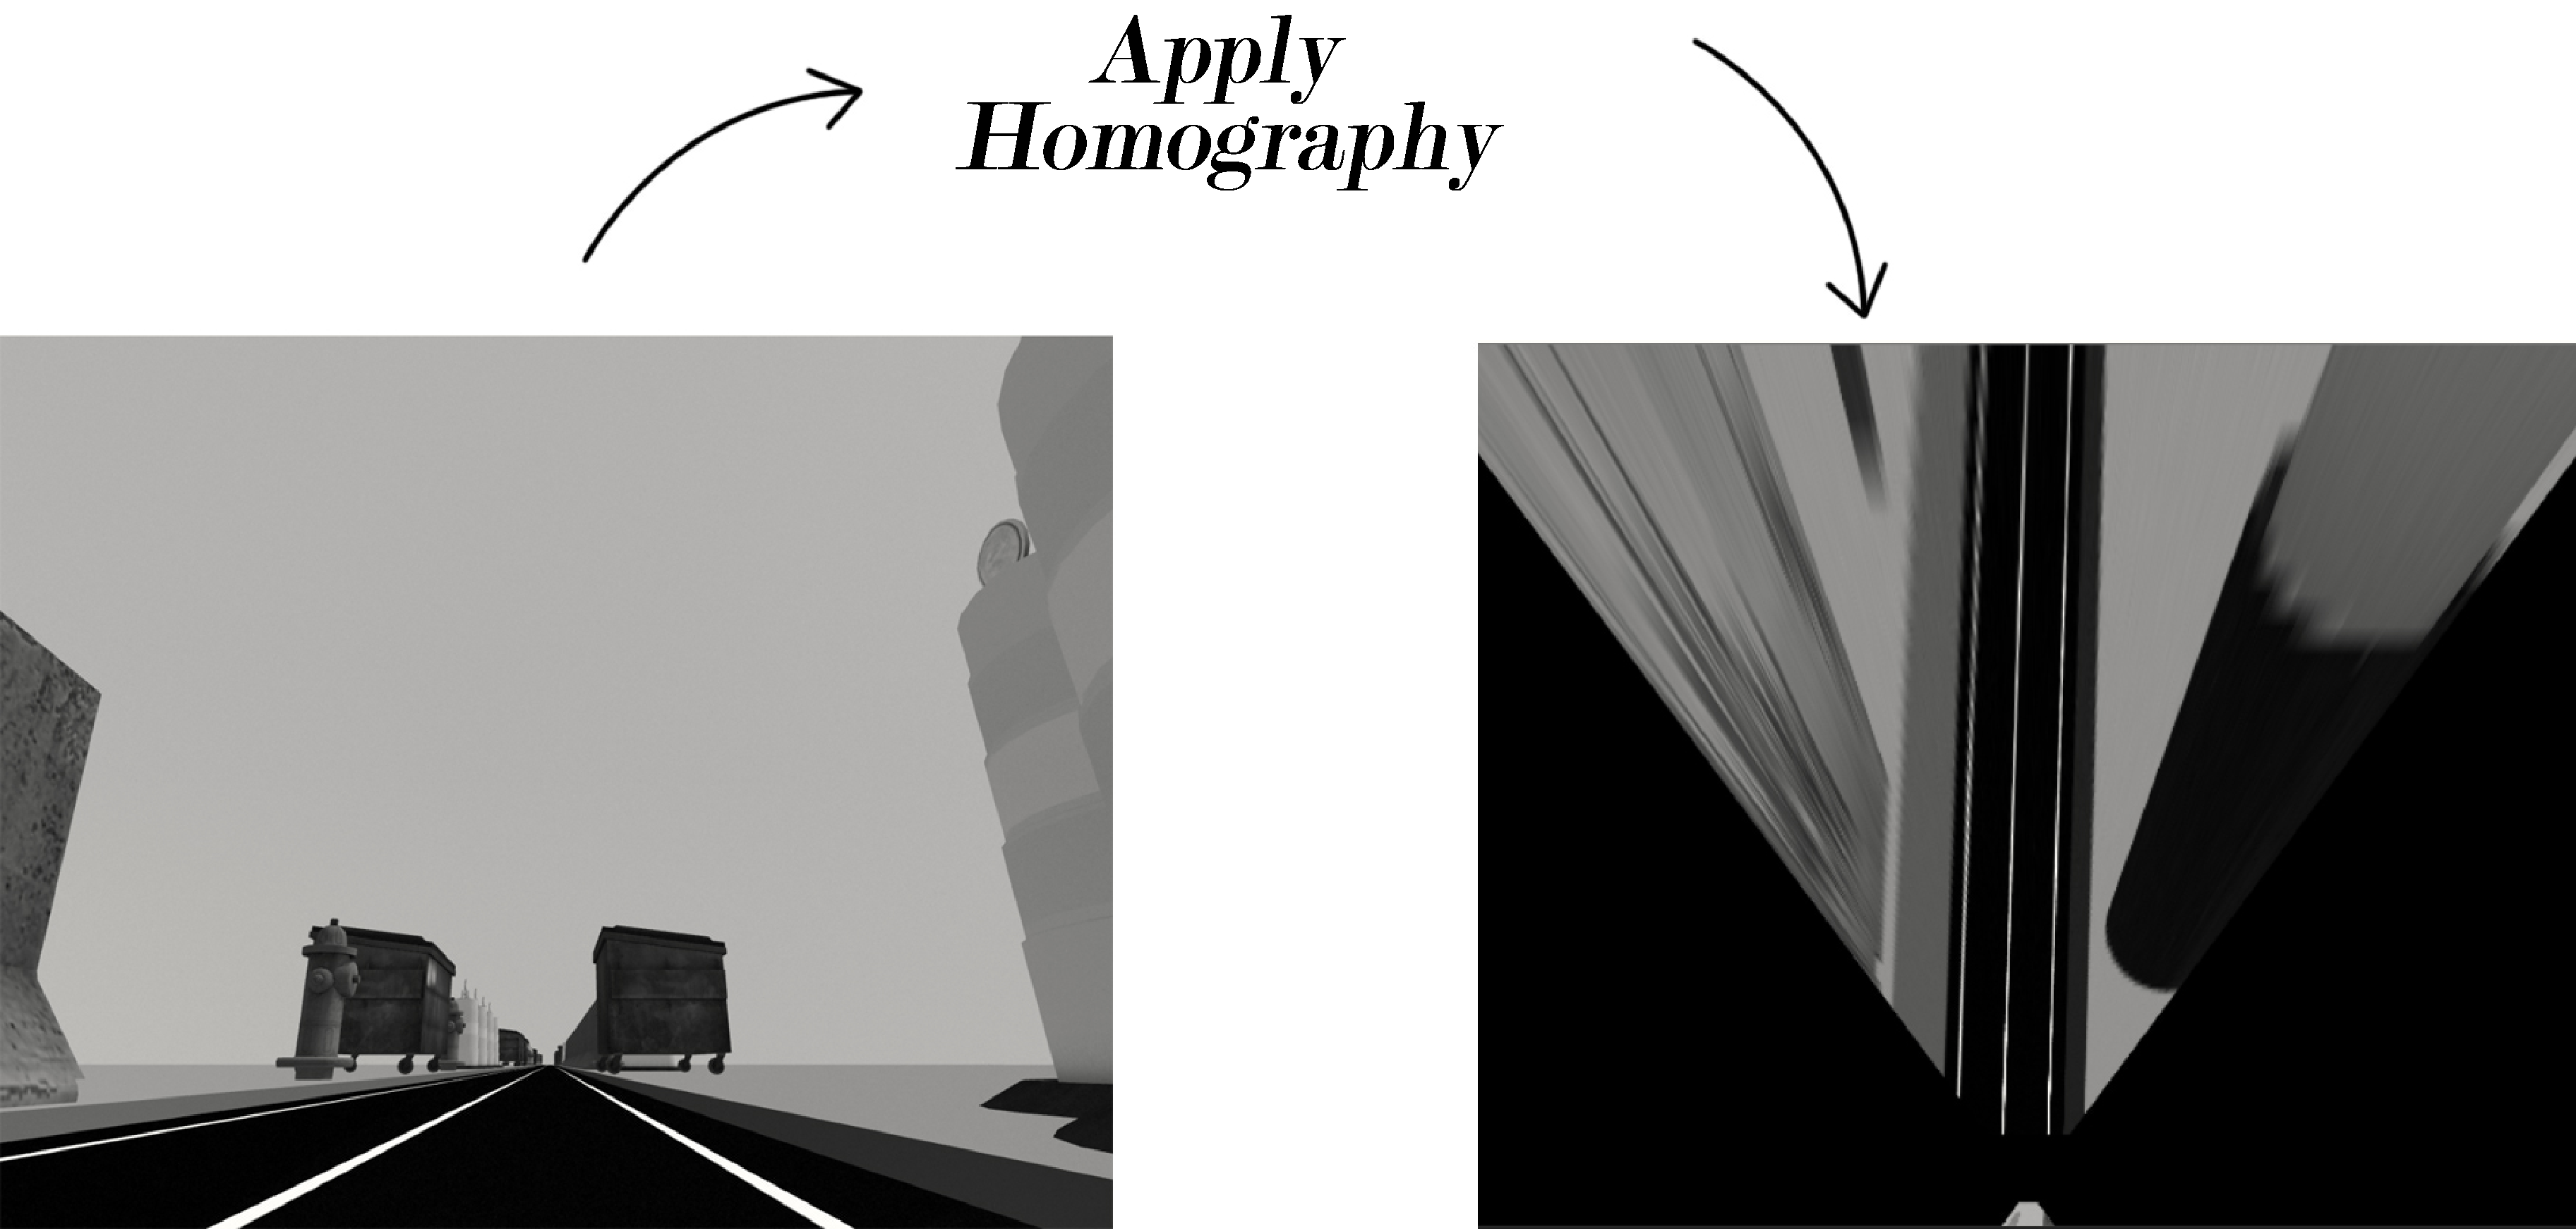
\includegraphics[width=\linewidth]{images/01-Apply-Homography.pdf}
    \caption{Applying homography on a raw grayscale image from the simulation, giving us our map (bird's eye view) view.}
    \label{fig_apply_homog}
\end{figure}


\begin{figure}[h]
    \centering
    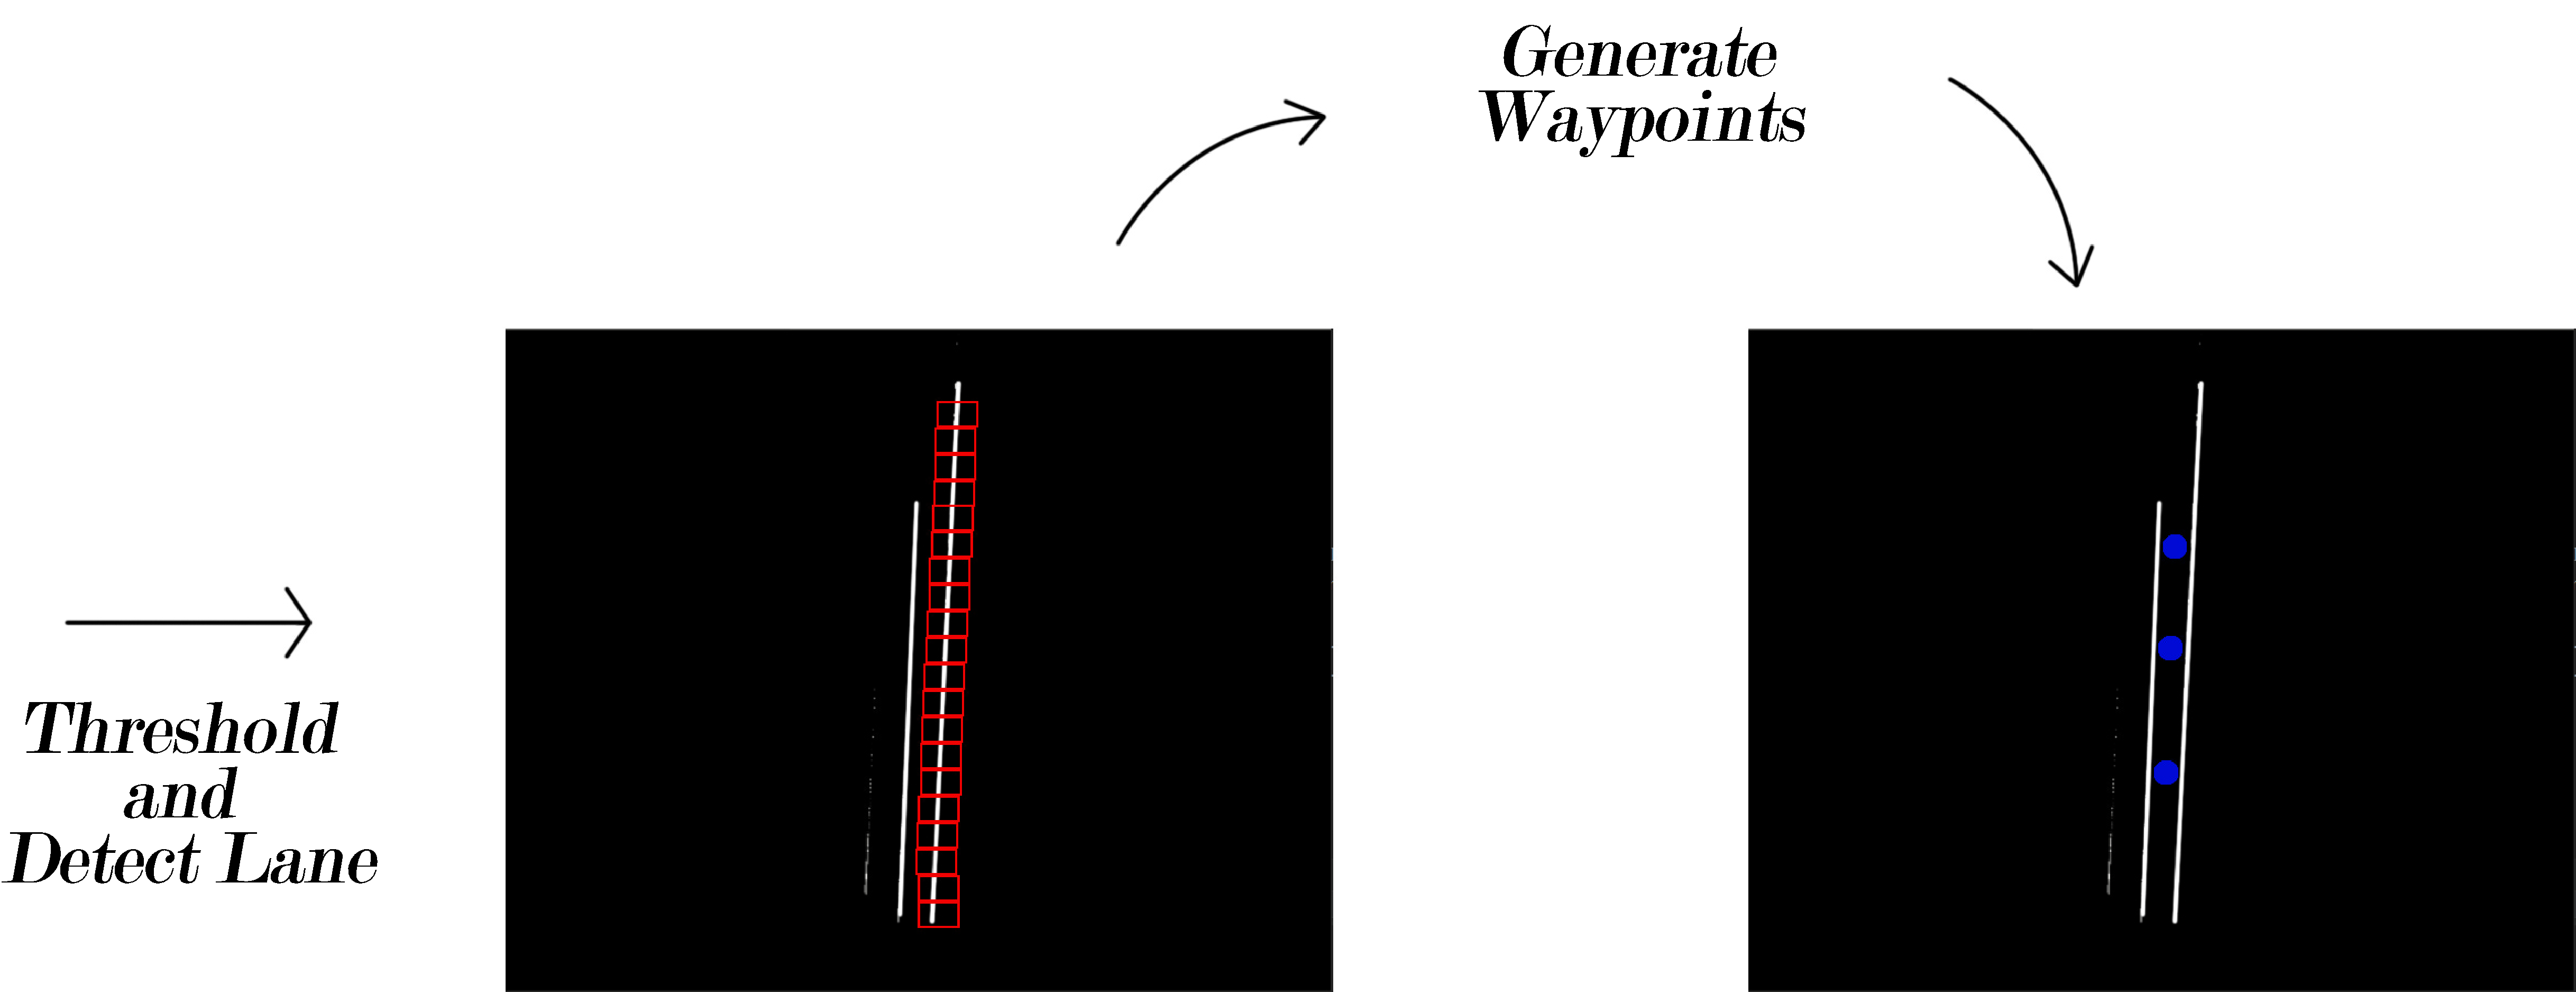
\includegraphics[width=\linewidth]{images/02-Generate-Waypoints.pdf}
    \caption{Detecting the lane on a thresholded bird's eye view image using sequential rectangles (shown in red), followed by generating way-points (blue dots) from the calculated quadratic equations of both the left and right lanes. }
    
    \label{fig_gen_wapoints}
\end{figure}


\begin{figure}[h]
    \centering
    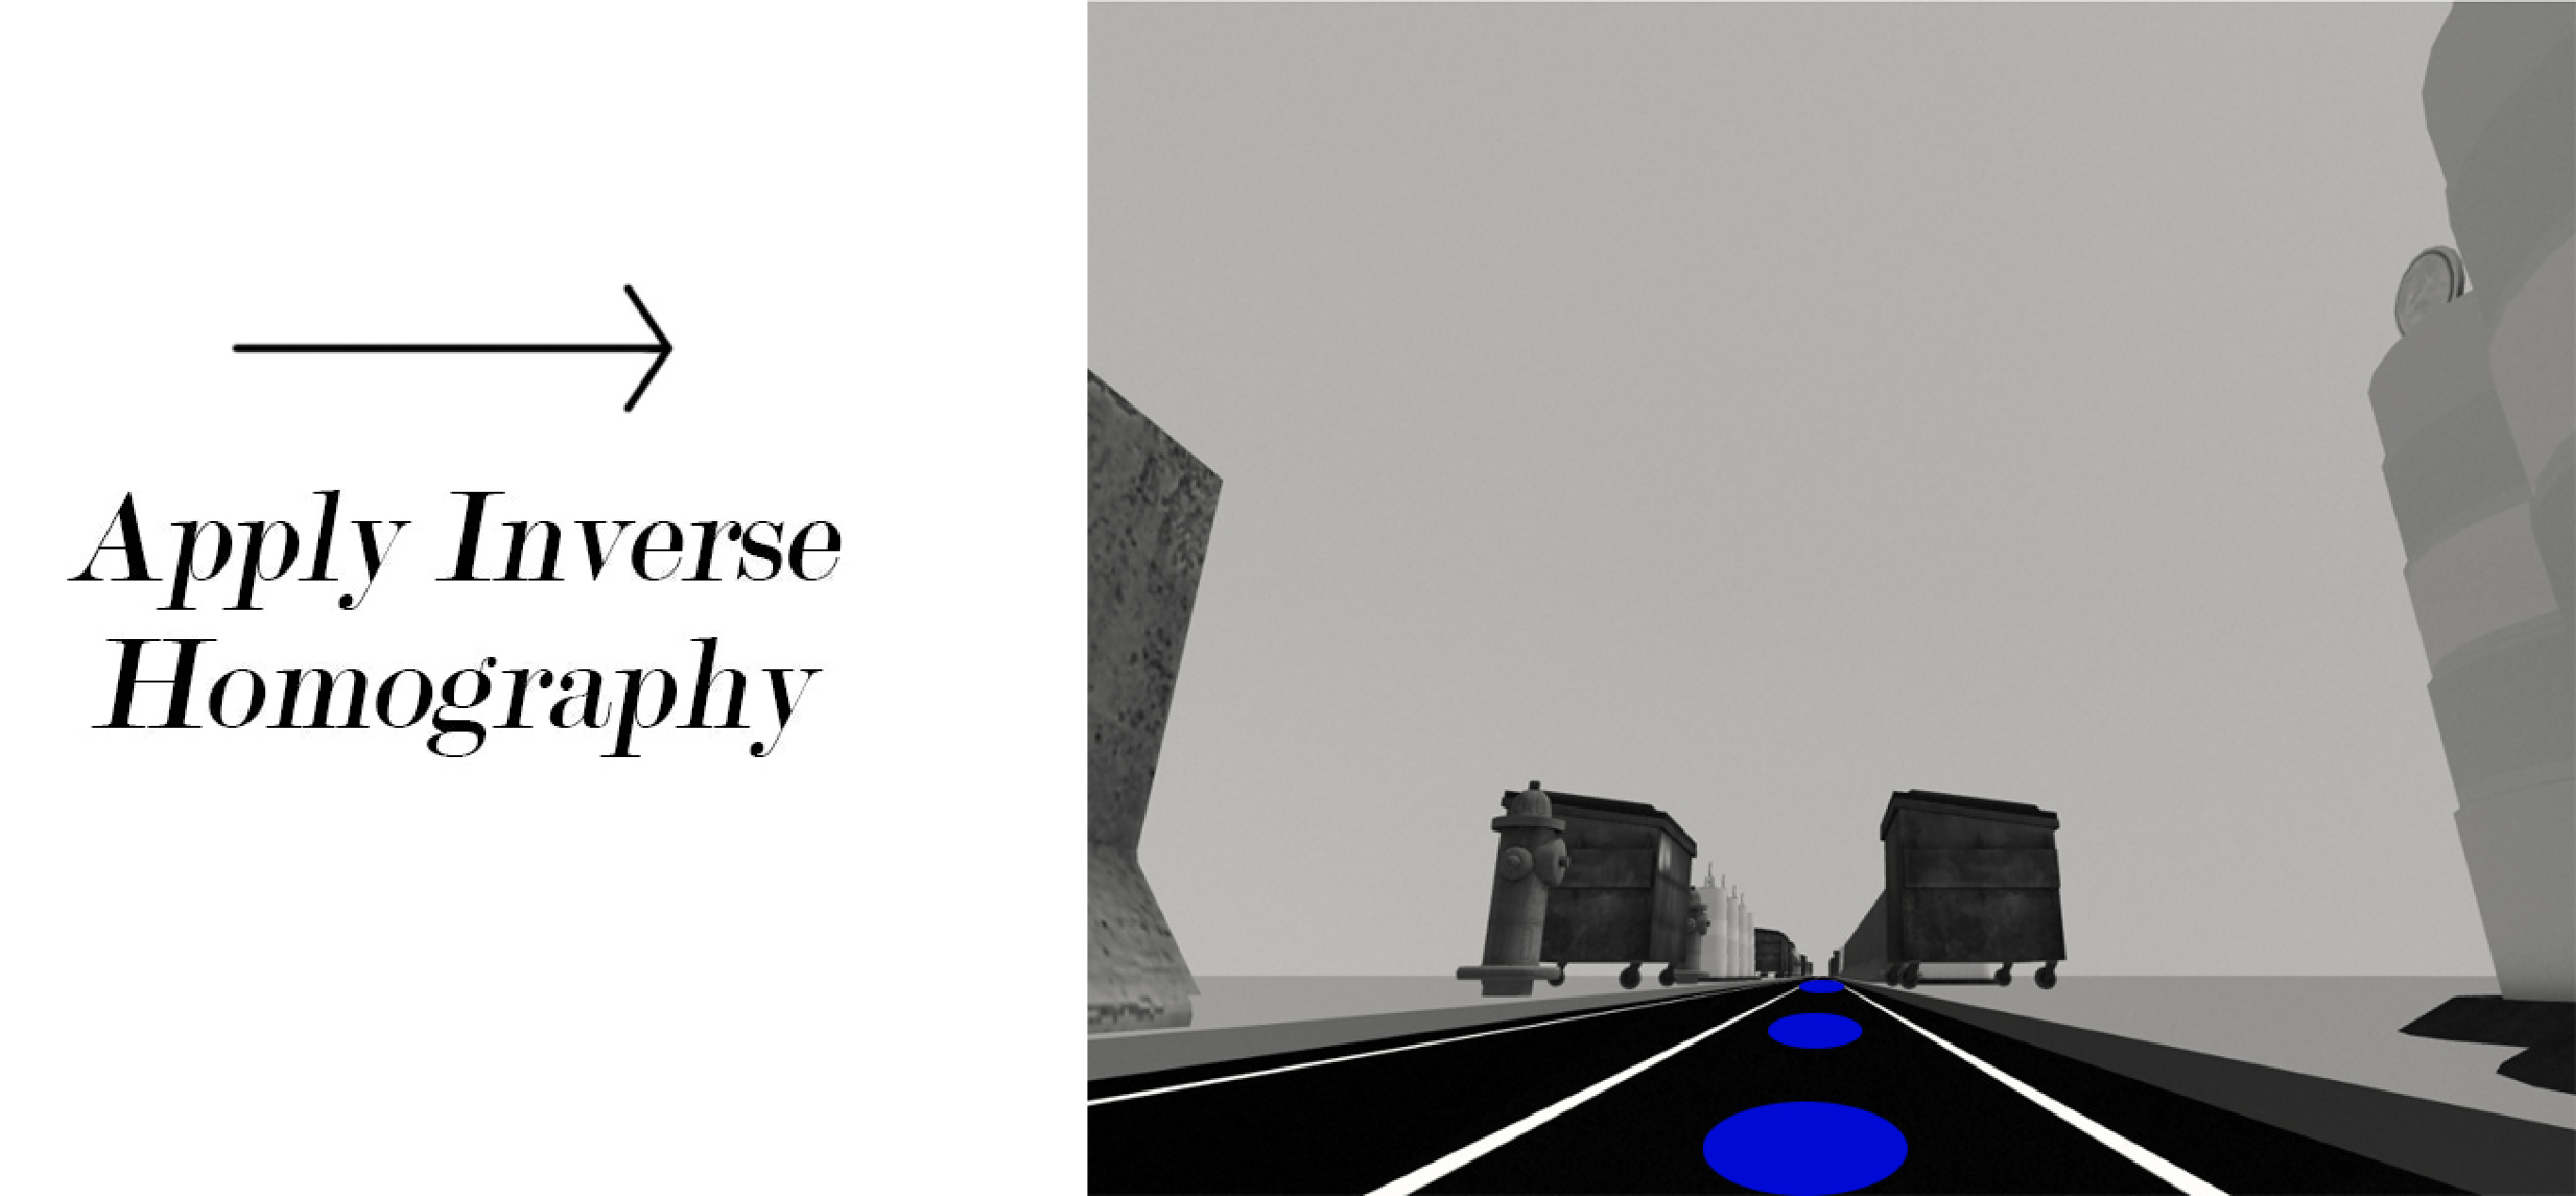
\includegraphics[height= 5cm]{images/03-Apply-Inverse-Homography.pdf}
    \caption{Applying inverse homography on the way-points generated in the bird's eye view to retrieve them in the simulation coordinate system.}
    \label{fig_apply_inv_homog}
\end{figure}





\subsection{Lane Changing}
\label{method_lane_change}
In this sub-section, we provide the implementation details of our lane changing module previously discussed in \ref{specs_lane_change}.We make use of the V2V communication and assume that the surrounding vehicles to the ego one will take the worst case scenario actions over the coming time-steps. 
We  assume that the ego vehicle is in a certain lane and there are other four hypothetical vehicles in hypothetical positions A, B, C, and D as described in figure \ref{fig_LC_diagram}.

\begin{figure}[!h]
    \centering
    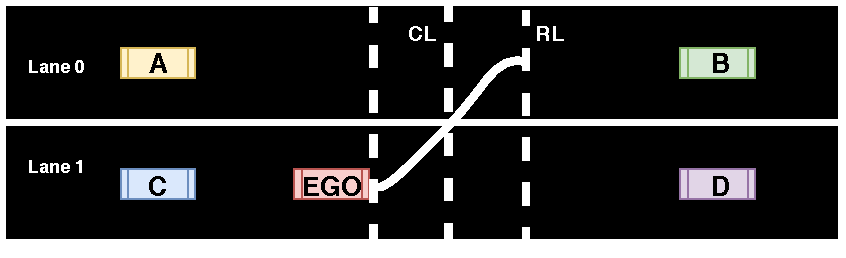
\includegraphics{images/LaneChangeDiagram.pdf}
    \caption{Lane Change schematic diagram.}
    \label{fig_LC_diagram}
\end{figure}
\leavevmode
Where:
\begin{conditions*}
 Lane 0    &   to go lone; where the ego vehicle is going to change lane to it \\
Lane 1    &  current lane; where the ego vehicle exists \\
Centerline    &  the line corresponding to half the distance taken to make the lane change action \\
Rightline    &  the line corresponding to the point where lane change action will be finished \\
A    &  vehicle position in the to go lane ; where it is located before the center-line \\
B    &  vehicle position in the to go lane ; where it is located after the center-line \\
C    &  vehicle position in the current lane ; where it is located before the center-line \\
D     &  vehicle position in the current lane ; where it is located after the center-line \\
\end{conditions*}

As mentioned before, the velocity ranges from 0 to 0.5 \(m/s\) with 0.1 \(m/s\) step. i.e:[0 0.1 0.2 0.3 0.4 0.5].
The lane change action is executed in a certain time and distance for each velocity, these results were calculated empirically in Table  \ref{table:LC_vel_dist_time}.
\\ 
\begin{table} [h]
\begin{center}
\begin{tabularx}{1\textwidth} { 
  | >{\centering\arraybackslash}X 
  | >{\centering\arraybackslash}X 
  | >{\centering\arraybackslash}X
  | >{\centering\arraybackslash}X
  | >{\centering\arraybackslash}X | }
 \hline
 Velocity (\(m/s\)) & Total time taken to finish lane change action (\(sec\)) & Total distance taken to finish lane change action (\(m\)) & Half the  distance taken to finish lane change action (\(m\)) & 
Time taken to reach the center-line , reach half the total distance (\(sec\))
 \\
 \hline
 0.1  & 15  & 1.367 & 0.681 & 7  \\
 \hline
 0.2  & 9  & 1.631 & 0.819 & 4  \\
 \hline
 0.3  & 6  & 1.754 & 0.984 & 3  \\
 \hline
 0.4  & 4  & 1.855 & 1.108 & 2  \\
 \hline
 0.5  & 4  & 1.976 & 1.23 & 2 \\
\hline
\end{tabularx}
\caption{Lane change time and distance at certain velocities.}
\label{table:LC_vel_dist_time}
\end{center}
\end{table}
\leavevmode
\\ 
\textbf{Assumptions:}

\begin{enumerate}
\item Lane change occurs at the instant velocity of the ego vehicle. 
\item Lane change action is executed in N time-steps where the time-step is lane change execution action time divided by the delta time.
\item The descriptive parameter is not the whole time-steps, it is half the time-steps; number of time-steps taken by ego vehicle to reach center-line. For simplicity we will conveniently say that half the time-steps is “time-steps” as we don’t use the whole time-steps as a parameter in any calculations. 
\end{enumerate}
\textbf{Algorithm Core:}
\\ \\
The algorithm starts with finding the existing vehicles in the environment, vehicles may be A, B, C or D. We are not concerned with vehicle C as it will not affect the lane change action as we will explain later on. \\
\\
To know whether there is a vehicle D or not, we simply make use of the V2V communication and check whether there is a vehicle in the same lane and ahead of the ego vehicle. We keep looping over all the vehicles that are in the same lane and ahead of the ego vehicle till we find the nearest one to the ego vehicle and this is considered our vehicle D. \\
\\
The case for vehicles A and B is different because if any of the two vehicles accelerate or decelerate too much this may change it from position A to B or vice versa.  \\
To make sure that a vehicle is B we assume that the vehicle applies maximum deceleration during all time-steps the ego vehicle takes to reach center-line, if its position is ahead of the centre-line then it is B. Otherwise, we assume the vehicle applies maximum acceleration during all time-steps the ego vehicle takes to reach center-line, if its position is behind the centre-line then its A. Also, there is a case where we can’t decide if the vehicle is for sure A or B so we return that lane change is infeasible. This part of the algorithm being handled in the code is isSafeWRTD() and isAorB() functions. \\
\\
After getting all the information related to vehicles in the environment surrounding the ego vehicle, we check for the feasibility of executing the lane change action and whether it is safe or not. This is done by assuming that every vehicle will make the worst case scenario affecting the lane change action and then determine the feasibility of executing the lane change action. \\
\\ 
In case of vehicle C, it will not affect the ego vehicle by any means as it will follow it by Krauss model. It will adapt its velocity with the ego vehicle and keep a minimum safe distance accordingly. \\
\\ 
In case of vehicle D, the possible actions that vehicle D can do is to accelerate, decelerate or stop. In case of acceleration there will be no problem because it will be out of the ego’s vehicle window and will not affect its lane change action. \\
In case of deceleration, we assume the worst case vehicle D will make. The worst case here is to perform maximum deceleration during the time-steps, number of time-steps taken by ego vehicle to reach center-line. If the hypothetical position of vehicle D becomes before the center-line, therefore lane change action is not feasible. \\
In case of the stop action, it is implicitly handled in the deceleration action case because if the vehicle decelerates several times till it stops this will end up as if we are handling the stop action from the very beginning. So if the vehicle stops and is found to be before the center-line this will make the lane change also infeasible. This part of the algorithm being handled in the code is isSafeWRTD() function.\\
\\
In case of vehicle B, vehicle B is in the target lane for the ego vehicle so there are two cases to handle considering the hypothetical velocity and position, these cases are calculations before reaching the center-line and calculations after reaching the center-line. In the first case, before reaching the center-line, we assume that vehicle B will perform maximum deceleration during the time-steps and make sure it is still considered to be at hypothetical position B. In the second case, we calculate the number of time-steps taken by the ego vehicle to reach the right-line (starting from center-line) and assume max deceleration during these time-steps. If the final hypothetical position of vehicle B is before the right-line then lane change action is infeasible. If it is after the right-line then we check the feasibility using Krauss model by calculating the maximum possible safe velocity between the ego vehicle and vehicle B and check if the velocity of the ego vehicle is greater than the maximum safe velocity then lane change action is not feasible, otherwise it is feasible. This part of the algorithm being handled in the code is in isSafeWRTB() function. \\
\\
In case of vehicle A, since vehicle A is also in the target lane for the ego vehicle then it has two cases to handle; before and after reaching the center-line. In the first case, before reaching the center-line, we assume that vehicle A will perform maximum acceleration during the time-steps and make sure it is still considered to be at hypothetical position A. In the second case, after the ego vehicle reaches the center-line, we check whether the relative velocity between ego vehicle and vehicle A is safe (using Krauss model) by calculating the maximum possible safe velocity between the ego vehicle and vehicle A and check if the velocity of vehicle A is greater than the maximum possible safe velocity then the lane change is not feasible, otherwise it is feasible. This part of the algorithm being handled in the code is in isSafeWRTA() function. \\




%-----------------------------------------------------%
\subsection{Path Planning}
\label{method_path_plan}
In this sub-section, we provide the implementation details of our AV's path planning module introduced in \ref{specs_path_plan}. Our work was based on ROS navigation stack \cite{ROS_nav_stack}. However, we need to tune its used parameters such as max acceleration and max velocity in both angular and linear directions. Moreover, we use the default parameters for the TEB local planner \cite{ROS_TEB_local_planner} except for the goal tolerance parameter. We increase the goal tolerance parameter; to make the AV start to decrease its velocity before reaching the goal with safe distance, to ensure it stops exactly at the goal position.\\ \\
As for our two adjustments to the module previously highlighted in \ref{specs_costmap} and \ref{specs_custom_planner}, the following provide a summary of the details of their implementation.

\begin{enumerate}
    \item \textbf{Adding a Communication Costmap Layer}
    \\ \\
    Before getting into the details of the functionalities that our newly added costmap layer has to be able to perform, it helps to understand the mechanism by which each of the individual layers in the ordered list of costmap layers contributes to the final generated master costmap which is eventually used in the path planning.

    Each of the costmap layers, except the inflation layer, holds its own copy of grid cells which are each marked as either LETHAL, if the cell is known to have an obstacle, NON LETHAL, if the cell is known to be free, or NO INFORMATION, if the state of the cell is unknown to this layer. For a single update of the master costmap, the two following passes through the ordered list of layers are taken \cite{costmap}:
    
    \begin{enumerate}
        \item \textbf{Update Bounds Pass:}
        The aim of this first pass is to determine how much of the master costmap layer has to be updated in this round. Consequently, the pass starts with an empty bounding box and iterates, in order, over the costmap layers \cite{costmap}. Each layer expands this box as appropriate, resulting in a final bounding box representing the whole area of the master layer that has to be updated.
        \item \textbf{Update Costs Pass:}
        The aim of this second pass is to perform the actual update of the costs of all the grid cells of the master layer that are within the bounding box specified in the first pass \cite{costmap}. Again, the layers are iterated over in order, and each of them uses the costs of its copy of the grid cells to update the cost of all master grid cells within the bounding box \cite{costmap}. There are different ways in which this update step could be executed. As one example, layers which come later in the ordered list can be allowed to overwrite the costs specified by the previous layers or not. Accordingly, the order of the layers in the list and the update method adopted affect the final generated master layer and how it can be interpreted.
    \end{enumerate}
    
    Based on the explained update mechanism, it is important that we choose the order of our communication layer in the list of costmap layers, as well as the update method to be used in the update costs step. The mostly used order of the other three layers is: 1. Static Layer 2. Obstacle Layer 3. Inflation Layer \cite{costmap}. Since we are confident about the communication data encoded in our communication layer, we might want it to overwrite cost values specified by either the static layer or the obstacle layer. However, we want the inflation layer to add a buffer zone around the cells marked as LETHAL by our new layer as well. Hence, we choose that the order of the costmap layers is as follows: 1. Static Layer 2. Obstacle Layer 3. Communication Layer 4. Inflation Layer. As for the method of updating costs adopted by our communication layer, we choose that it overwrites the cost of the master cells with ONLY the valid costs in its copy of grid cells; where only the LETHAL and NON LETHAL labels are considered valid. This means that the cost of master cells are not overwritten by any cells marked as NO INFORMATION in our layer’s copy of the grid cells.
    \\ \\
    Therefrom, there are two main functionalities that our communication layer should be capable of performing apart from the actual extension of the bounding box (during the update bounds pass) and the actual update of costs of the master layer grid cells (during the update costs pass). These functionalities are:
    
    \begin{enumerate}
        \item Setting the costs of its own copy of grid cells based on the communicated positions of other vehicles within its communicated range.
        \item Determining which region of its copy of grid cells has changed since the last update pass of the master layer. This is necessary so that it can, during the update bounds pass, increase the size of the bounding box accordingly.
    \end{enumerate}
    
    In order to perform these functionalities, the communication layer needs the following inputs and parameters:

    \begin{itemize}
        \item \textbf{Inputs:}
        \begin{enumerate}
            \item \textbf{List of Vehicles' Footprints:} This is a list of all the footprints of vehicles that are currently within the vehicle’s communication range, where the footprint is the corner coordinates of the rectangular region occupied by the vehicle in the map. Since the vehicle’s communication module already allows it to keep a list of all the data of vehicles in its communication range, as thoroughly discussed in \ref{method_comm_rec}, this list of footprints is already available to the vehicle.
            \item \textbf{Last Marked Region:} This is in the form of coordinates of a rectangular region resembling the area within which exist all the cells in the layer’s copy of grid cells which were marked as LETHAL in the last update pass. The communication layer already keeps track of these coordinates during each pass; therefore they are always known to it.
            \item \textbf{Vehicle Position:} The communication layer could be chosen to be part of a global layered costmap, used by the global planner in generating the global path, or to part of a local layered costmap, used by the local planner in generating the local path. While the global layered costmap and its origin are static, the local layered costmap is \textbf{rolling}. This means that the origin of the local layered costmap and all its layers should always be at the center of the vehicle. Therefrom, in case the communication layer is added to a local layered costmap structure, the current vehicle position needs to be known to the layer so that its origin gets updated accordingly. This is obtained from the vehicle’s LiDAR sensor.
        \end{enumerate}
        \item \textbf{Parameters:}
        \begin{enumerate}
            \item \textbf{Is Rolling:} This is a boolean parameter indicating whether the origin of the layered costmap should be at the vehicle’s center at all times. This is the case with the local layered costmap but not the global one.
            \item \textbf{Safety Clearing:} When the layer clears the cost of cells previously marked as LETHAL, it could be prompted to clear some extra meters around these cells to enhance robustness. This parameter specifies those extra meters.
        \end{enumerate}
    \end{itemize}
    
    When first created, the communication layer is initialized with a copy of the grid cells of the master layer. The costs of all the cells are initially NO INFORMATION. Next, using the above inputs and specified parameters, the communication layer performs the following steps during every update pass of the master layer:

    \begin{enumerate}
        \item If the “is rolling” parameter is true, this means the communication layer is part of a layered costmap that is rolling; whose origin has to be the vehicle’s center at all times. In this case, the origin of the communication layer is updated to coincide with the current coordinates of the vehicle. This is necessary so that any coordinates specified in the map frame could be directly mapped to coordinates in the costmap layer.
        \item Given the corner coordinates of the last marked region, the communication layer clears this region in its copy of the grid cells by setting these cells’ cost to NO INFORMATION. This is to clear any costs from the previous update pass. For robustness purposes, the rectangular region to be cleared is inflated by the amount specified by the safety clearing parameter.
        \label{red_box_pt}
        \item Upon receiving the updated list of vehicle footprints, the layer marks all those cells as LETHAL in its copy of the grid cells.
        \label{mark_pt}
        \item The layer then stores the coordinates of the rectangular region within which all those cells marked as LETHAL exist.
        \label{green_box_pt}
        \item Now that the marking and clearing have been completed, and upon receiving the coordinates of the bounding box during the update bounds pass, the communication layer increases the box’s bounds as appropriate. It includes the marked region whose coordinates are stored in \ref{green_box_pt}, and the cleared region in \ref{red_box_pt}, whose coordinates are those of the marked region from the previous path plus the safety clearing buffer.
        \label{yellow_box_pt}
        \item During the update costs pass, the communication layer simply overwrites the costs of the master grid cells within the final bounding box with those stored in its copy.
    \end{enumerate}
    
    For further clarification, steps \ref{red_box_pt} - \ref{yellow_box_pt} are summarized in figure \ref{fig:costmap_fig}. Lightly shaded cells are cells marked as LETHAL in the previous update pass, and resemble vehicles’ footprints at that time. Darkly shaded cells are cells marked as LETHAL in the current update pass, and resemble the current vehicles’ footprints. The safety clearing parameter is set to 0 meters in this example for simplification.
    
    \begin{figure}[hbtp]
    \centering

    \begin{subfigure}[t]{0.3\textwidth}
        \centering
        
\includegraphics[width=1\linewidth, height=2.5cm]{Costmap1}
        \caption{Red box bounding the previously marked region (\ref{red_box_pt}).}
        \label{fig:red_box_fig}
    \end{subfigure}\hfill
    \begin{subfigure}[t]{0.3\textwidth}
        \centering
        
\includegraphics[width=1\linewidth, height=2.5cm]{Costmap2}
        \caption{Clearing the previously marked region (\ref{red_box_pt}).\\}
        \label{fig:clear_fig}
    \end{subfigure}\hfill
    \begin{subfigure}[t]{0.3\textwidth}
        \centering
        
\includegraphics[width=1\linewidth, height=2.5cm]{Costmap3}
        \caption{Marking newly received vehicle footprints (\ref{mark_pt}).\\}
        \label{fig:mark_fig}
    \end{subfigure}\hfill
    
    \begin{subfigure}[t]{0.3\textwidth}
        \centering
        
\includegraphics[width=1\linewidth, height=2.5cm]{Costmap4}
        \caption{Green box bounding the currently marked region (\ref{green_box_pt}).\\ \\}
        \label{fig:green_box_fig}
    \end{subfigure}\hfill
    \begin{subfigure}[t]{0.3\textwidth}
        \centering
        
\includegraphics[width=1\linewidth, height=2.5cm]{Costmap5}
        \caption{Yellow bounding box received by layer during the update bounds pass (\ref{yellow_box_pt}).\\}
        \label{fig:yellow_box1_fig}
    \end{subfigure}\hfill
    \begin{subfigure}[t]{0.3\textwidth}
        \centering
        
\includegraphics[width=1\linewidth, height=2.5cm]{Costmap6}
        \caption{Yellow bounding box expanded accordingly and new red bounding box saved for the next pass (\ref{yellow_box_pt}).}
        \label{fig:yellow_box2_fig}
    \end{subfigure}\hfill

    \caption{Communication Layer Update Algorithm}
    \label{fig:costmap_fig}
    \end{figure}
    
    
    \item \textbf{Adding a Custom Planner for Lanes:}
    \begin{itemize}
        \item \textbf{Inputs:} 
        \begin{enumerate}
            \item The AV's current position
            \item The AV's local planner path (An array of poses)
            \item If the AV has already started lane changing
            \item If the AV has finished lane changing
        \end{enumerate}
        \item \textbf{Outputs:} The control actions:
        \begin{enumerate}
            \item Lane Keeping
            \item Left Lane Changing
            \item Right Lane Changing
        \end{enumerate}
        \item \textbf{Parameters:} Refer to \ref{specs_env_agent_mdl}
        \begin{enumerate}
            \item The y-coordinates of the separating lines between lanes
            \item The x-coordinates of the lanes indicating their lengths 
            \item Lanes numbers
        \end{enumerate}
        \item \textbf{Algorithm:\\} 
        \begin{algorithm}[H]
\SetAlgoLined
Determine which lane the AV is positioned at: by getting the AV's position through localization module then getting its location relative to lanes using their coordinates.\;
Determine which lane the AV is heading to: by getting the last pose in the local planner trajectory and getting its location relative to lanes as well.\;
Communicating with the navigation module to know if the AV has started lane changing if it was ordered to do so.\;
\If{It has already started lane changing}{
     do not send other lane changing goals in order for the AV to change its lane only once then wait for the next action. Send lane keeping goals instead for the AV to separate two lane changes with lane keeping for one time stamp\;}
\uIf{It has not already started lane changing}{
     \uIf{The heading lane is greater than the current lane}{
     Output left lane changing.\;}
     \uElseIf{The heading lane is smaller than the current lane}{Output right lane changing.\;}
     \uElseIf{Both lanes are the same}{Output Lane Keeping.\;}
     }
\caption{Adding a Custom Planner for Lanes}
\end{algorithm}
    \end{itemize}
\end{enumerate}

%-----------------------------------------------------%

\subsection{Navigation}
\label{method_nav}
In this sub-section, we go through our designed system for the navigation module previously discussed in \ref{specs_nav}. \\ \\
The default action in the navigation module is lane keeping, the AV has to keep moving until it reaches the goal. It only stops if it is stuck. 
\begin{itemize}
    \item \textbf{Inputs:} 
    \begin{enumerate}
        \item The chosen action in any time stamp by the path planning module (\ref{specs_path_plan}).
        \item A Boolean indicating if the AV has already reached the goal.
    \end{enumerate}
    \item \textbf{Output:} The AV performs one action in any given time stamp. 
    \item \textbf{System Components:} A master that handles three clients:
    \begin{enumerate}
        \item Lane Keeping Server Client
        \item Velocity Control Server Client
        \item Lane Changing Server Client
    \end{enumerate}
    \item \textbf{Server-Client Communication Type}
        \begin{enumerate}
            \item \textbf{Goal}: It contains information about:
                \begin{enumerate}
                \item \textbf{Control Source:} The control source, whether it came from navigation module or an external command. (\ref{specs_ext_cmds}).
                \item \textbf{Control Action:} Lane Keeping or Lane Change.
                \item \textbf{Direction:} Changing lane left or right in case of lane changing control action.
                \item \textbf{Acceleration:} The acceleration in case of lane keeping in case of lane keeping control action.
                \end{enumerate}
                %-----------------------------------------------------%
    \item \textbf{Feedback}: If the control action is feasible or not.
    \item \textbf{Result}: If the control action is completed or not due to infeasibility.
        \end{enumerate}
        \item \textbf{System Algorithms: }
        \begin{itemize}     
            \item \textbf{Servers: }
            After receiving goals: 
                \\ \\
        \end{itemize}
            %-----------------------------------------------------%
            \begin{algorithm}[H]
                \SetAlgoLined
                \While{While preemption from the client is not requested}{
                Listen to the \textbf{velocity} requested from velocity controlling server in a stream of messages that changes every time stamp\;
                Start lane keeping using \ref{method_lane_keep}, and \ref{method_long_ctrl} modules\;
                }
                Stop lane keeping\;
                Send the result to the navigation master\;
                \caption{Lane Keeping Server Algorithm}
            \end{algorithm}
            %-----------------------------------------------------%
            \begin{algorithm}[H]
                \SetAlgoLined
                \While{While preemption from the client is not requested}{
                Get the requested velocity from the local planner in \ref{specs_path_plan}\;
                Execute \ref{method_long_ctrl} module to check its feasibility and adjust it to be feasible if it wasn't;
                Send the velocity to lane keeping server\;
                }
                Stop generating velocities\;
                Send the result to the navigation master\;
                \caption{Velocity Controlling Server Algorithm}
            \end{algorithm}
            %-----------------------------------------------------%
            \begin{algorithm}[H]
                \SetAlgoLined
                Check whether the lane change in the requested direction is feasible\;
                  \eIf{The lane change is feasible}{
                     Execute lane change using \ref{method_lane_change} module\;
                    Send result to the navigation master indicating that the lane changing is finished\;
                    }{
                    Send feedback and result to the navigation master indicating lane changing was not feasible\;
                    }
                \caption{Lane Changing Server Algorithm}
            \end{algorithm}      
            %-----------------------------------------------------%
            \begin{itemize}
            \item \textbf{Navigation Master:}
            The high-level control master module (\ref{method_high_lvl_cntrl}) listens to the path planning module that generates a control action every time stamp, and pass the chosen control action to the navigation module master.
            \end{itemize}
            \begin{algorithm}[H]
                \SetAlgoLined
                For every time stamp, a thread is generated by the high-level control master in section (\ref{method_high_lvl_cntrl}) \cite{ROSBookMorgan} and executes this algorithm\;
                  \eIf{The navigation master is deactivated $\lor$ \\
                  \hspace{0.35cm} The AV has already reached the goal $\lor$\\
                  \hspace{0.35cm} The AV is currently executing lane change $\lor$\\
                  \hspace{0.35cm} The control action hasn't changed}
                  {Terminate this thread\;}
                  {
                  Check the control action\;
                    \uIf{The control action is lane keeping}
                    {
                    Send goals to lane keeping and velocity controlling servers\; 
                    Terminate this thread\;
                    }
                    \uElseIf{The control action is lane changing}
                    {
                    Send goal to lane changing server\;
                    Block the thread till the lane changing server sends feedback\;
                    \eIf{The feedback indicated that lane changing is infeasible}
                    {
                    \uIf{The AV hasn't been lane keeping already}
                    {Send goals to lane keeping and velocity controlling servers for the AV to start lane keeping\;}
                    Terminate the thread\;
                    }
                    {
                    Cancel all goals sent to lane keeping and velocity controlling servers\;
                    Send to the path planning module\; (\ref{method_path_plan}) that lane change is starting\;
                    Terminate this thread\;
                    }
                    }
                  }
                \caption{Navigation Master Algorithm}
            \end{algorithm} 
            %-----------------------------------------------------%
        
\end{itemize}
%-----------------------------------------------------%
\subsection{External Commands Following}
\label{method_ext_cmds}
In this sub-section, we explain the details of our designed system for the external commands following module previously discussed in \ref{specs_ext_cmds}. \\ \\
When the external commands following module is activated, there is no default actions unlike the navigation module \ref{method_nav}. An external system decides the action in any time stamp. The AV stops and wait until a suitable action is chosen.
\begin{itemize}
    \item \textbf{Inputs:}
    \begin{enumerate}
        \item Control action (Left lane change, Right lane change, Accelerate, Don't change velocity, Decelerate).
        \item Acceleration value.
        \item A Boolean to indicate if the external commands following module should end.
        \item Time needed to execute the control action if it was lane keeping.
    \end{enumerate}
    \item \textbf{Outputs:} 
    \begin{enumerate}
        \item A trial for command execution.
        \item Its feasibility.
        \item Time Taken if the command was executed. 
    \end{enumerate}
    \item \textbf{System Components:} The same servers in the navigation module (\ref{method_nav}) but with three different clients.
    \item \textbf{Server-Client Communication Type} The same communication type mentioned in the navigation module (\ref{method_nav}).
    \item \textbf{System Algorithms: }
    \begin{itemize}
        \item \textbf{Servers:}
            \begin{itemize}
                \item \textbf{Lane Keeping Server:} Same algorithm presented in the navigation module (\ref{method_nav})
            \end{itemize}
%-----------------------------------------------------%
            \begin{algorithm}[H]
                \SetAlgoLined
                Get the acceleration from the external commands following master\;
                \While{preemption from the client is not requested}{
                Check the feasibility for the new velocity given the acceleration value using \ref{method_long_ctrl} module\;
                \eIf{it was feasible}
                {Send the velocity to the lane keeping server for this time stamp\;
                }
                {\eIf{it was the first time stamp}
                {Send the result to the external commands following master indicating the action was not feasible at the first time stamp\;}
                {Break\;}
                }
                }
                Stop generating velocities\;
                Send the result to the external commands following master indicating the action was successful for at least one time stamp\;
                \caption{Velocity Controlling Server Algorithm}
                \label{Alg:velocityControllingRL}
            \end{algorithm}
%-----------------------------------------------------%
                \begin{itemize}
                \item \textbf{Lane Changing Server:} Same algorithm presented in the navigation module (\ref{method_nav})
            \end{itemize}
        \item \textbf{External Commands Following Master: } \\
        The high-level control initializes a thread in the external commands following master with a given control action. Therefore, the external commands following master executes the following algorithm. 
            \end{itemize}
%-----------------------------------------------------%
            \begin{algorithm}[H]
                \SetAlgoLined
                \uIf{the action is lane keeping}
                {Send a goal to the lane keeping server\;
                Send a goal to the velocity control server and block the thread for the required time\;
                Get the result from the velocity controlling server\;
                Calculate the execution time between sending the goal and getting the result\;
                Cancel the lane keeping goal\;
                Send the result and the execution time to the high-level control master\;
                Terminate\;
                }
                \uElseIf{the action is lane changing}
                {Send a goal to the lane changing server\;
                Block the thread till the feasibility is executed\;
                \eIf{lane changing was infeasible}
                {Send the result with zero execution time to the high level control master\;}
                {Block the thread till the lane change get executed\;
                Send the result with the execution time to the high level control master\;}
                }
                \caption{External Commands Following Algorithm}
                \label{Alg:external_cmds_follow}
            \end{algorithm}

\end{itemize}
 
%-----------------------------------------------------%
\subsection{High-Level Control Master}
\label{method_high_lvl_cntrl}
This sub-section discusses our implementation of our AV's high-level control master previously highlighted in \ref{specs_high_lvl_cntrl}. The following is a summary of the module's inputs, outputs and associated algorithm.

\begin{itemize}
    \item \textbf{Inputs: }
    \begin{enumerate}
        \item \textbf{First Communication Channel:} A Stream of messages sent by the path planning module (\ref{method_path_plan}).
        \item \textbf{Second Communication Channel:}
        \begin{itemize}
            \item A request sent by a server client connection with the external system that, at some point, will need to take control over the AV. The external system is \ref{method_collab_tech}.
            \item A Boolean to indicate whether external commands following module is activated or deactivated. 
        \end{itemize}
    \end{enumerate}
    \item \textbf{Outputs:} The AV should be controlled by only one module (navigation module or external commands following module) in any given time stamp.
    \item \textbf{Algorithm: }
    \end{itemize}
    %-----------------------------------------------------%
                \begin{algorithm}[H]
                \SetAlgoLined
                \While{the system is on}
                {
                Block the main thread until a message is received in any communication channel\;
                \uIf{a message is received in the first channel}
                {
                Generate a new thread and run the following\;
                Let the navigation module take control (\ref{method_nav})\;
                Send the control action to the navigation module \ref{method_nav}\;
                Wait till the navigation module terminate the thread\;
                }
                \uElseIf{a message is received in the second channel}
                {Generate a new thread and run the following\;
                \uIf{the external system asks to deactivate the external commands following module}
                {Activate the navigation module again\;}
                \uElseIf{the external system asks to execute a control action}
                {Deactivate the navigation module so that its concurrent threads will be terminated, refer to \ref{method_nav}\;
                Hand the control action to the external commands following module to execute it\;
                Wait for the external commands following module to send the control action's feasibility and time taken to be executed if it was feasible, refer to \ref{method_ext_cmds}\;
                Send the result to the external system client, such as \ref{method_collab_tech}\;}
                Wait for the external commands following module to terminate the thread\;
                }
                }
                \caption{High-Level Control Master Algorithm}
            \end{algorithm}
%-----------------------------------------------------%

\section{V2V Communication}
\label{method_v2v_comm}
In order to simulate our simple V2V communication system previously discussed in \ref{specs_v2v_comm}, each vehicle should be capable of both broadcasting its own identification data (ID) and receiving the ID of other vehicles within its communication range. 

\subsection{ID Message Structure}
\label{method_ID_struct}
The chosen contents of the communicated ID messages are as follows:

\begin{itemize}
    \item \textbf{Vehicle Type:} “racecar”/“EV”, according to our problem
    \item \textbf{Vehicle Position:} the x and y coordinates of the vehicle center in the map coordinates
    \item \textbf{Vehicle Lane:} an integer indicating the number of the lane in which the vehicle is, according to a preset convention
    \item \textbf{Vehicle Footprint:} the corner coordinates of the rectangular region occupied by the vehicle in the map
    \item \textbf{Vehicle Velocity:} the current velocity of the vehicle
    \item \textbf{Vehicle Maximum Velocity:} the maximum possible velocity of the vehicle
    \item \textbf{Vehicle Maximum Acceleration:} the maximum possible acceleration of the vehicle
\end{itemize}

\subsection{Broadcasting ID Messages}
\label{method_comm_send}
In order for each vehicle to broadcast its ID message, it needs the following inputs and predefined parameters:

\begin{itemize}
    \item \textbf{Inputs:}
         \begin{enumerate}
             \item \textbf{Vehicle Position:} This is obtained from the vehicle’s LiDAR sensor.
             \item \textbf{Vehicle Velocity:} This is obtained from the vehicle’s electronic speed controller (ESC).
         \end{enumerate}
    \item \textbf{Parameters:}
         \begin{enumerate}
             \item \textbf{Vehicle Maximum Velocity}
             \item \textbf{Vehicle Maximum Acceleration}
             \item \textbf{Vehicle Type}
             \item \textbf{Vehicle Dimensions:} The vehicle dimensions are needed so that the vehicle is able to calculate its footprint.
             \item \textbf{Lane Numbering Convention:} The convention of the lane numbering in the current map has to be known to the vehicle so that it can map its position coordinates to a lane number.
             \item \textbf{Vehicle Number:} This is a unique number assigned to each vehicle so that its broadcasted ID could be associated with it.
         \end{enumerate}
\end{itemize}
Using these inputs and specified parameters, the vehicle broadcasts its ID through the following steps:

\begin{enumerate}
    \item Using the vehicle’s coordinates in the map frame as well as its known dimensions, its footprint in the map is calculated.
    \item Knowing the lane numbering convention and the vehicle’s coordinates in the map, the vehicle’s lane number is calculated.
    \item All the information needed to construct the vehicle’s ID message are then ordered in a structured format and stamped by both the vehicle’s number and the current time at which it is broadcasting its ID.
    \item The vehicle then sends its ID message over a public communication channel accessible to the other vehicles. This communication channel, or topic, is one of the main communication styles supported by ROS. It is a unidirectional bus over which messages could be exchanged in an asynchronous manner \cite{ROSBookMorgan}.
\end{enumerate}

\subsection{Receiving ID Messages}
\label{method_comm_rec}
Since the topic over which vehicles send their ID messages is public, each vehicle can have access to the ID of all other vehicles in the environment. However, this does not match the realistic assumption that vehicles can receive messages from others only within their communication range. Consequently, to simulate the realistic scenario, vehicles discard messages sent by other vehicles beyond their communication range. Henceforth, the needed inputs and predefined parameters are:

\begin{itemize}
    \item \textbf{Inputs:}
         \begin{enumerate}
             \item \textbf{Vehicle Position}
             \item \textbf{New Communicated ID Message:} This is an ID message read by the vehicle from the public topic. The vehicle reads the ID messages one at a time, and it receives them ordered by the time at which they were broadcasted.
             \item \textbf{Last List of Other Vehicles’ IDs:} The vehicle keeps a list of IDs received by all other vehicles within its range. The last version of this list is needed as an input so that it can update it upon receiving a new ID message.
         \end{enumerate}
    \item \textbf{Parameters:}
         \begin{enumerate}
             \item \textbf{Vehicle Number}
             \item \textbf{Vehicle’s Communication Range:} This is the radius of the circular zone resembling the vehicle’s communication range. Broadcasted IDs of any vehicles beyond this zone cannot be known to the vehicle.
         \end{enumerate}
\end{itemize}

Using these inputs and specified parameters, the vehicle is able to update the list of IDs associated with all vehicles in its communication range. This is done through the following steps:

\begin{enumerate}
    \item The vehicle reads an ID message from the public topic.
    \item Since the vehicle itself has also sent its ID over the same topic, it has to first check that the ID message it just read does not belong to it. If it does, then the vehicle should ignore this message. This is done by comparing the vehicle number of the sender with the vehicle’s own number.
    \item With the knowledge of the vehicle’s coordinates in the map and the coordinates incorporated in the received ID message, the vehicle calculates the distance between the sender vehicle and itself. If this distance exceeds the radius of the vehicle’s communicated range, this means that the sender vehicle is currently outside the accessible range. Hence, if the last ID of this sender vehicle was previously stored in the list of IDs, it should be deleted. If it was not, then this newly received message is discarded.
    \item If the sender vehicle is found to be within the vehicle’s communication range, then this newly received ID is added to the list of IDs. If the sender vehicle’s last ID was already stored in the list of IDs, then its ID should be updated instead.
\end{enumerate}

This guarantees that a simple V2V communication system is simulated such that, at all times, each vehicle has an updated list of the IDs of only the vehicles that are within its specified communication range.

%-----------------------------------------------------%

\section{Cooperation Technique}
\label{method_collab_tech}
In this section, we provide the implementation details of our adopted cooperation technique previously described in \ref{specs_collab_tech}.

\subsection{Single Agent Problem Formulation}
\label{method_single_agent_pf}
In a typical reinforcement learning problem, the agent learns how to perform a certain task by interacting with the environment.  Concept-wise, it observes the environment .Then it takes an action accordingly. As a result, it receives a reward from the environment. Code-wise, the agent observes the system state which is composed of agent state and the environment state. Then, it chooses an action from a pool of feasible actions according to action choice paradigm. The environment executes that action i.e. it applies changes that result from that action. The environment then returns: an observation which is the system's new state, a reward of a value determined according to whether the agent’s picked action yields favorable results or not, a done flag to indicate whether the episode has been terminated or not, and other information that is not used in training but important such as goal state which is the state at which the episode terminates. If done is false, the episode has not been terminated, hence the loop will continue. In order to formulate any problem as an RL problem, we need to define an environment, system states, agent actions, and reward function. 


\subsubsection{Environment}
\label{sumo_env_SA}
Environment is an urban road which is divided into lanes . Each lane is discretized into cells. Two entities co-exist inside the environment: the Emergency Vehicle (EV), and the agent which is an autonomous vehicle. The EV is not a trainable agent. It drives using a car-following-model all the time and does not use our RL model to drive.  Refer to Section \ref{sumo_agent_model} for more information about the used car-following-model. The justification is that the EV has the highest priority and should not change its predetermined plan for any other vehicle. According to its car-following-model, it picks a value of five possible acceleration values at every time step. Possible acceleration values are integers in the range of [-2, 2]. This range could be altered. However, we are just concerned about making it limited to 5 possible values for the sake of our Q-Table. Acceleration values affect velocity range which in return affects system states size. The overgrown states size makes the training process significantly more demanding and sometimes intractable, especially using non–deep learning RL models. The agent is a trainable/learning vehicle and was trained using the Q-learning algorithm to evacuate the road for the EV to help it reach its destination within optimal time .\\

\subsubsection{States}

The observed state is the one used for training: the one that is used to index the Q-Table. It is composed of EV velocity, EV lane, agent velocity, agent lane, and the EV position relative to agent if the EV is within agent’s window. If it is outside the agent's window, then y position will be denoted by a cut-off value which represents whether it is in front of or behind EV. Agent window represents the perception and proximity area around the agent where it can detect the existence of the EV and receive rewards for its actions. \\ \\
The following value ranges are scenario-specific and could be altered with wider or narrower ranges. Our goal was to make training affordable by limiting states size. EV velocity is an integer in the range of [0, 10]. So the maximum velocity for the EV is 10 cells per time step . Agent velocity is an integer in the range of [0, 5].   EV and agent lanes could be any lane of the three lanes, indexed as {0, 1, 2}. \\ \\ 
The hidden state is only known to the environment itself. It contains all information in observed state besides goal global coordinates, and EV global coordinates. It is used to check for episode termination. If the EV position is the same as the goal position, the episode will terminate.The episode terminates if any case of the following three cases happens: First, if EV has reached its goal position. Second, if the agent has finished its trip. Third, if maximum number of time-steps has reached to stop infinite episode occurrence.
\subsubsection{Actions}
Actions encompass agent’s possible driving actions.  Agent’s possible actions are : acceleration,  deceleration,  change lane to the left,  change lane to the right, and continue as it is (no speed nor lane change is involved). We  check  feasibility  of  all  actions  given  a  certain  state. This is possible as number of possible states and actions is known, limited in size and more importantly feasibility check in SUMO is not a time consuming process. We could visualize this as state action space, that is reduced to feasible state action space which is determined at the beginning before model get trained.

\subsubsection{Reward}

Designing a reward function was the most challenging part of the problem formulation. We were willing to design reward function that rewards results rather than behaviors which is a common mistake as illustrated in \cite{russell2016artificial}. These results should be always desirable .A well formulated reward function should reward/penalize activity, passivity and do nothing towards side effects. Activity means that agent actively takes an action to give way to EV. Passivity is when the agent does not take any action that blocks EV way. Side effects mean actions done by the agent that do not affect EV in a way or another. There are two types of reward : step reward and final reward.
\begin{itemize}
    \item 
    Step reward is the reward that agent takes every time-step. We have designed it to be a linear function of EV acceleration at every time-step as increasing speed of EV is always a desirable result.  Then we have edited it to be a weighted linear function of EV acceleration and agent’s actions. The main reason for this edit was to make sure that our agent drives safely and stops its oscillating behavior. Refer to Section \ref{single_agent_results} for more information about step reward phases and associated results with every phase until we have managed to make agent behavior an optimal one.
  \item 
  Final reward is the reward given to the agent when the episode terminates. We have designed it to be a linear function of the ratio between actual EV travel time taken until episode has terminated and optimal travel time. Optimal time is the time taken by EV if it has always managed to drive with its max speed during the episode. At first, we believed it will be useful to introduce final reward to our problem formulation design. However, we have discovered later on that it is not suitable for our problem design. The reason was the lack of a method to divide this reward over pairs of states and actions along the episode fairly in a way that represents their contribution to the success of failure of the agent. Especially if some of agent actions over certain episode were wise enough to efficiently evacuate road for the EV while other actions are not. There was no way to give every action its corresponding portion of final reward. For this concern, we have disabled the final reward and  made reward design only limited to step reward.
 

    
\end{itemize}

\subsubsection{General Problem Formulation Design Considerations}
Besides designing states, actions, and reward, there are other vital design considerations: 
\begin{itemize}
    \item \textbf{Interaction Guarantee} 
    \label{meth_SA_int_guarantee}
    
    \item \textbf{Agent window }
    
    \item \textbf{Dynamics Handling} 
    
\end{itemize} 


\noindent Agent training process is totally dependent on its interaction with environment and corresponding rewards it receives during this interaction. In case of training single agent, interaction is represented only in agent interaction with the EV. We have generated random initialisation of both agent and EV lanes, positions, and relative distances. However, this random initialization ensures that there is sufficient interaction time and distance before EV reaches its goal. So how is this interaction guaranteed?
\begin{itemize}
    \item Vehicles’ initial positions in their lanes are ordered according to their maximum velocity.  For instance, if the maximum velocity of agent is less than EV maximum velocity, then agent will be inserted in the lane ahead of EV to ensure interaction. 
    
    \item Given that the maximum velocity of every vehicle is known and goal position is determined, we calculate upper bound on time at which EV and agent must meet before EV reaches its goal using the following inequality :
    \begin{equation}
    maximum\,velocity_{faster\,vehicle} * time_{meeting} <position_{goal}
    \end{equation}
    
    \item According to the upper bound of their meeting time, we calculate the upper bound of meeting position using the following inequality :
    \begin{equation}
        position_{meeting} + maximum\,velocity_{slower vehicle}*time_{meeting}<position_{goal} 
    \end{equation} 
    
\end{itemize} 
\noindent
Agent window represents the perception and proximity area around the agent where it can detect the existence of the EV and receive rewards based on how its actions have affected EV acceleration. We have utilized the concept of agent window for three reasons: 
\begin{enumerate}
    \item To keep state space fixed even if road or lanes are infinite as part of observed state is the relative position between agent and EV with the agent being the origin. If EV is inside agent’s window, its position will be represented as a relative position to agent. If it is outside window, it will take one of two states which represents whether EV is in front or behind agent. In other words, if the EV is outside the agent's window and behind it by hundred cells, it is exactly the same as being behind it by a thousand cells.
    
    \item To reward agent for activity, passivity, and do nothing towards side effects. If EV is inside the agent window, the agent will receive reward based on how its active and passive actions affect the EV reward. If EV is outside agent window, it means that agent and EV are too far to affect each other. Hence, the reward will update the value function of this metaphorical state-action pair that represents any EV outside window. 
    \item Defining a window around agent where the agent is the origin makes agent perspective a centric one. Agent-centric perspective is better in learning policies that generalize better \cite{Ye2020RotationTA}. \\ 
\end{enumerate}

\noindent We have simplified dynamics by assuming that the road is divided into lanes where every lane is discretized into cells so there is no meaning for lateral movement within the lane itself, but rather there is only longitudinal movement within the lane. This is aided by the assumption that lane keeping and lane change functionalities are to be handled by the AV capabilities.  Consequently, we have assumed that once agent has decided to change lane, it will be in that lane in the next time-step. Our focus at this stage was to train the agent on how to cooperate with the EV not how to drive. This was our plan to simplify dynamics. It was impressive to figure out that SUMO holds the same principles about handling dynamics, refer to Section \ref{sumo_agent_model} for information about how Sumo handles dynamics. Also, we have considered dynamics along with cooperation in our ROS implementation thoroughly.




\subsection{Moving the Single Agent to Multi-Agent Environment}
Placing the Single-Agent model in a Multi-Agent environment was done to test it. We wanted to evaluate our model's performance when placed with other vehicles. Several clarifications are in order here:
\begin{enumerate}
    \item Several minimal code changes were made. Mainly, the episode did not terminate upon the agent exiting the road; as there were many agents now and our goal was to observe the EV behaviour not train the agent. Also, instead of the RL Algorithm being a global variable to the system, each vehicle now had its own control Algorithm (one of those mentioned in \ref{sumo_agent_model}).
    
    \item The agent vehicle is still not able to integrate any position/velocity related parameters with its RL decision making process. It still consults the Q-Table using the earlier clarified observed state of itself and the EV only. The agent, however, has knowledge about which actions are feasible and which are not, based on the states of the other agents.
    
    \item Control over the number of vehicles on the road and the percentage of AVs using each model was introduced, allowing to conduct controlled experiments and observe the effect of different parameters on the travel time. More details on this in Section \ref{sec:RL_Results}.
\end{enumerate}

%-----------------------------------------------------%
\section{System Integration}
\label{method_integr}
After developing the autonomous functionalities of our vehicles, we aim at deploying the single-agent RL model we designed in SUMO (\ref{method_single_agent_pf}) on one of our agent vehicles in the presence of an EV in Gazebo. In general, we adopt the same conventions relating to the agent-environment interactions. However, owing to the much more realistic nature of the Gazebo simulation environment, several changes had to be introduced. These changes deal with real-time constraints, dynamics of the AV, and system latency. These changes are summarized in the following points:

\begin{enumerate}
    \item In the original model, the action to be taken at each time step is chosen, either using the exploit or the explore policy, from a set of \textbf{only the current feasible actions}. This was possible then because SUMO handled the feasibility calculations in a reasonable amount of time. On the contrary, with the complexity in dynamics and the system as a whole in Gazebo, calculating the feasibility of all the different actions at every time step is an extremely time-consuming process that would introduce an undesirable lag to the simulation and adds latency. This is besides the fact that it is not realistic to perform the  checking of all actions’ feasibility in such a regular manner. As a result, we resorted to choosing the action to be taken from the set of “all” actions and checking this chosen action’s feasibility. If it is found to be feasible, then it gets executed and if it is not, another one is chosen. This is repeated till a feasible action is found and taken. 
    \item Since our system in Gazebo is meant to mimic a real one, the agent vehicle’s window should be within the limits of its communication range at all times. This is essential in order for the vehicle to be able to receive the data broadcasted by the EV so that it can use it in its model.
    \item The velocity ranges assigned to the agent and the EV were changed to [0, 0.5] and [0, 1] respectively. This is because our vehicle’s controllers were tuned to those ranges.
    \label{vel_ranges_pt}
    \item One of the major assumptions in the implementation on SUMO is that each of the different actions of the agent get executed in a single time-step. This means that the vehicle takes one time-step to complete its action regardless of whether it is a simple “accelerate” action or a complex “lane change” one. This is certainly unrealistic; a lane change action, for instance, will definitely require more time to get executed than other actions. Moreover, the time taken to change the lane depends on the vehicle’s velocity during this maneuver. \\ \\
    As a result of such difference, actions taking longer to get executed seem to buy the emergency vehicle extra time in which it could accelerate, if possible. Accordingly, since the agent’s reward mainly depends on the change in the emergency vehicle’s velocity as a result of the agent’s action execution, higher reward values might end up being associated with longer actions. This means that the agent might falsely learn to prefer certain longer actions. To resolve this issue, we modified the agent’s reward function such that the reward is normalized by the time taken to execute the corresponding action.
    \label{all_one_sec_pt}
    \item Adding to \ref{all_one_sec_pt}, in order to reduce the huge difference in the actions’ execution times, we associated the simple “accelerate”/”decelerate”/”no acceleration” actions with a certain time period in which to be taken. In other words, the new action is “accelerate for \(x\) seconds” instead of merely “accelerate”. All the same, if any action was found to be infeasible any time during the specified time period, the action is simply aborted and the reward calculated based on the actual execution time it took.
    \label{timed_actions_pt}
    \item As a result of \ref{timed_actions_pt}, we modified the acceleration ranges of the agent, and accordingly of the emergency vehicle, to be of lower values. The reason for this modification is that, now that the agent is asked to accelerate/decelerate for longer time periods, we do not want it to reach its maximum/minimum velocities during the execution of a single action. Consequently, based on our velocity ranges in \ref{vel_ranges_pt}, our chosen acceleration ranges for the agent and the EV are [0, 0.0167] and [0, 0.0333] respectively.
    \label{acc_ranges_pt}
    \item Based on the decreased values of acceleration/deceleration in \ref{acc_ranges_pt}, for both the agent and the EV, the number of possible velocity values within the allowed range increased. This led to a considerable increase in the size of our Q-Table.
    \item Owing to the fact that our simulation on Gazebo is much more realistic than that on SUMO, the system is more susceptible to crashing as a result of the different existing uncertainties. Thus, we added another reason for which the episode can be forced to terminate: “simulation’s death”. If this happens, all the Q-Table updates which occurred in the last episode are discarded.
    \item The track simulated in Gazebo is shorter than the one in SUMO in order to avoid having very long episodes. However, the interaction between the agent and the emergency vehicle is still guaranteed in the same way discussed in \ref{meth_SA_int_guarantee}.
\end{enumerate}
Apart from the above mentioned adjustments, all other assumptions in the problem formulation were kept the same.
\\ \\
According to, \ref{specs_integr}, our system can be divided into three main entities: the RL algorithm, the environment, and a master managing the system interactions. The responsibilities and provided services associated with each of the entities are summarized in the following subsections:

\subsection{RL Algorithm}
    Since our adopted algorithm is Q-Learning, the master can request the following from the RL algorithm module:
        \begin{itemize}
            \item \textbf{Create/Load/Save/Update Q-Table}
            \item \textbf{Take Action:} 
            \end{itemize}
                \begin{algorithm}[H]
                \SetAlgoLined
                Generate an array that have the all actions\;
                \While{While a feasible action is not found in the array}{
                Pick an action\;
                Send it to the high-level control master to execute it, refer to \ref{method_high_lvl_cntrl}\;
                Get its feasibility and time taken\;
                \eIf{the picked action was feasible}{Send the action and time taken to master}{Remove the infeasible action from the array}
                }
                \caption{Taking Action Algorithm}
            \end{algorithm}
            \begin{itemize}
            \item \textbf{Disengage:}
            This is requested when the emergency vehicle exits the agent’s window, in which case, the RL algorithm is prompted to notify the high-level control master (\ref{method_high_lvl_cntrl}) to deactivate the the external commands following in (\ref{method_ext_cmds}).
        \end{itemize}

\subsection{Environment}
    Several services can be requested by the master from the environment. Those services include:
        \begin{itemize}
        \item \textbf{Start/Reset/Close Simulation:} The track in Gazebo and the vehicle models together constitute our simulation. The master requests that the simulation is started at the beginning of either training or testing the RL model, reset between episodes and closed at the end of session. For optimization purposes during the resetting of the simulation, the vehicle models are deleted and regenerated in the track but the Gazebo simulator itself is not restarted unless it has crashed. This is detected by a secondary thread in the environment module which frequently pings the simulation and indicates when it has crashed. This thread is also the one indicating that the episode needs to end for the reason “simulation death”.
        \item \textbf{Get Agent’s State:} The full states of all the vehicles, agent and emergency vehicle in our case, are known to the environment. Upon request, the environment returns the agent’s observed state.
        \item \textbf{Calculate Agent’s Reward:} With the action execution time as an input, the environment calculates and returns the agent’s normalized reward.
        \end{itemize}
        Aside from these services, the environment also continuously sends information to the master through a communication channel (topic). This information includes whether the emergency vehicle is inside or outside the agent’s window; accordingly whether the master should request the disengagement of the RL model. The environment also publishes to the master the status of the current episode: whether or not it has finished and for what reason.
        
\subsection{Master}
    As previously mentioned, the master is the maestro connecting the whole system together. Algorithms \ref{rl_on_ros_master_train_alg} and \ref{rl_on_ros_master_episode_alg} summarize its role in training the RL model. \\
    
            \begin{algorithm}[H]
                \SetAlgoLined
                Request "Start Simulation" from \textbf{Environment} and block till it is ready\\
                Run first episode using algorithm
                \uIf{episode ended because simulation died}{Prompt the \textbf{RL Algorithm} to discard Q-Table updates of this episode}
                \ref{rl_on_ros_master_episode_alg}\\
                \While{maximum number of episodes is not exceeded}{
                    Request "Reset Simulation" from \textbf{Environment} and block till it is ready\\
                    Run another episode using algorithm \ref{rl_on_ros_master_episode_alg}\\
                    \uIf{episode ended because simulation died}{Prompt the \textbf{RL algorithm} to discard Q-Table updates of this episode}
                    }
                Request "Close Simulation" from \textbf{Environment}\\
                Prompt \textbf{RL Algorithm} to save Q-Table
                \caption{Master Training Algorithm}
                \label{rl_on_ros_master_train_alg}
            \end{algorithm}
                
            \begin{algorithm}[H]
                \SetAlgoLined
                \While{\textbf{Environment} did not signal the end of episode}{
                    \uIf{\textbf{Environment} signaled that emergency vehicle is outside agent's window}{Prompt the \textbf{RL Algorithm} to declare disengagement\\
                    Block till \textbf{Environment} signals that the emergency vehicle is inside agent's window $\lor$ episode has ended}
                    \uIf{\textbf{Environment} signaled that episode has ended}{Break}
                    Request agent's initial state from \textbf{Environment}\\
                    Let \textbf{RL Algorithm} prompt taking action\\
                    Request agent's final state from \textbf{Environment}\\
                    Request calculation of agent's reward from \textbf{Environment}\\
                    Prompt \textbf{RL Algorithm} to update Q-Table
                }
                \caption{Master Episode Algorithm}
                \label{rl_on_ros_master_episode_alg}
            \end{algorithm}